% Problem 4.3: Monte Carlo integration (I)
% Notes and checklist: ../Exercises/4.03-mc-integration-1/README.md
% Figures:            \includegraphics{4.03-mc-integration-1/figures/<name>}
\exercise{3}{Monte Carlo integration (I)}

The integral to estimate is
\begin{equation}
  \mathcal I = \int_{\mathbb R^3} e^{-r^2/2}\,(x+y+z)^2\,dx\,dy\,dz, \qquad r^2 = x^2+y^2+z^2 .
\end{equation}
The Gaussian factor serves as the sampling density (importance sampling) and $(x+y+z)^2$ as the
function to average \cite{Carlon2025}. All runs use seed~1; the Gaussian numbers come from
\texttt{scipy.stats.norm.rvs}.

\subsection{Analytical value}

Expanding $(x+y+z)^2 = x^2+y^2+z^2 + 2(xy+yz+zx)$, every cross term is odd in at least one
coordinate and integrates to zero against the even Gaussian. Each square term gives
$\int x^2 e^{-x^2/2}dx \cdot \big(\int e^{-y^2/2}dy\big)^2 = \sqrt{2\pi}\cdot 2\pi = (2\pi)^{3/2}$, so
\begin{equation}
  \mathcal I = 3\,(2\pi)^{3/2} = 6\sqrt2\,\pi^{3/2} = 47.249 .
\end{equation}
A symbolic integration with \texttt{sympy} gives the same result.

\subsection{Estimate with Gaussian random numbers}

The Gaussian factor is not normalised: $e^{-r^2/2} = (2\pi)^{3/2}\,w(\mathbf r)$, where
$w(\mathbf r) = (2\pi)^{-3/2}e^{-r^2/2}$ is the density of three independent $\mathcal N(0,1)$ numbers.
Hence
\begin{equation}
  \mathcal I = (2\pi)^{3/2}\,\avg{f}_w \approx \mathcal I_N = \frac{(2\pi)^{3/2}}{N}\sum_{i=1}^{N} f(\mathbf r_i),
  \qquad f = (x+y+z)^2 ,
\end{equation}
with $\mathbf r_i$ drawn from $w$. The points are independent, so the standard error is
$(2\pi)^{3/2}s_f/\sqrt N$, with $s_f$ the sample standard deviation of the $f(\mathbf r_i)$.

\kulbox[5pt]{With $N = 10^6$ Gaussian points: $\mathcal I_N = 47.241 \pm 0.067$, compared with the
exact $\mathcal I = 47.249$, a deviation of $-0.12$ standard errors.}

\subsection{Variance of the estimate}

The central limit theorem predicts $\sigma^2(\mathcal I_N) = (2\pi)^3\,\mathrm{Var}_w(f)/N$. Here
$s = x+y+z \sim \mathcal N(0,3)$, so $s^2/3$ follows a $\chi^2_1$ distribution with variance 2, and
$\mathrm{Var}(f) = \mathrm{Var}(s^2) = 9 \cdot 2 = 18$. This gives
$\sigma^2(\mathcal I_N) = 18\,(2\pi)^3/N = 4465/N$.

To measure the variance we repeat the whole estimate $M = 1000$ times with independent points, for
13 values of $N$ from 10 to $10^5$, and take the sample variance of the 1000 values $\mathcal I_N$.
That variance is itself uncertain, with relative error $\sqrt{2/(M-1)} = 4.5\,\%$. A weighted fit of
$\ln\sigma^2$ against $\ln N$ (figure~\ref{fig:4.3-variance}) gives
\begin{equation}
  \sigma^2(\mathcal I_N) = 4441\,N^{-1.000 \pm 0.004},
\end{equation}
in agreement with the predicted exponent $-1$ and prefactor 4465. The product $N\sigma^2$ lies
between 4067 and 4750 for all $N$, each value with an error of about 200.

The spread of the individual values $f(\mathbf r_i)$ does not decrease with $N$; only the spread of
their mean does. The error $\sigma_f/\sqrt N$ is independent of the dimension of the integral: the
problem only enters through the prefactor $\sigma_f$, which depends on the chosen density.

\begin{figure}[htbp]
  \centering
  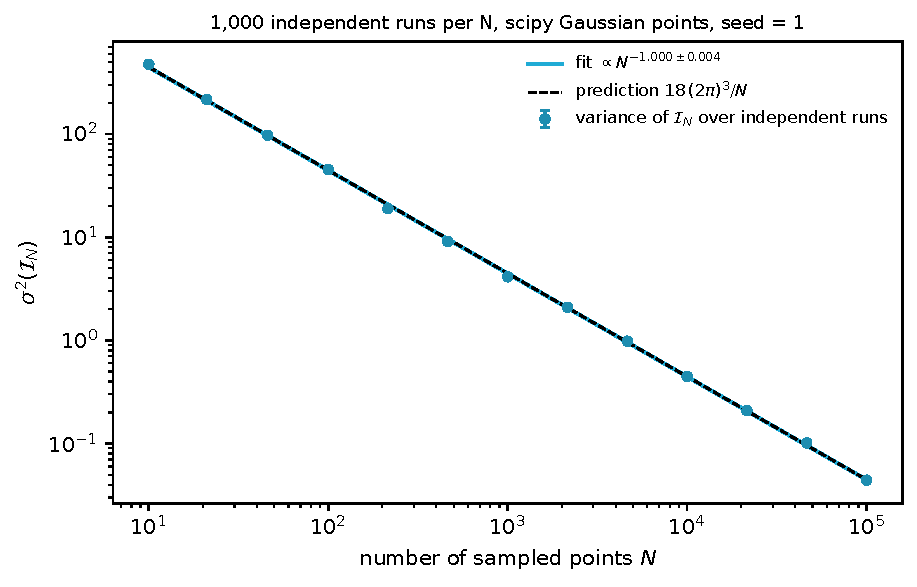
\includegraphics[width=0.75\linewidth]{4.03-mc-integration-1/figures/mc_variance}
  \caption{Variance of the importance-sampling estimate $\mathcal I_N$ over $M = 1000$ independent
    runs per $N$, for 13 log-spaced $N$ from 10 to $10^5$. Error bars $\sigma^2\sqrt{2/(M-1)}$. Line:
    weighted power-law fit; dashed: prediction $18\,(2\pi)^3/N$. Seed 1.}
  \label{fig:4.3-variance}
\end{figure}

\subsection{Why the two factors cannot be swapped}

Using $(x+y+z)^2$ as the density and $e^{-r^2/2}$ as the function to average fails for a basic
reason: a probability density must be non-negative \emph{and} normalisable. The first condition
holds, but $\int_{\mathbb R^3}(x+y+z)^2\,d^3r = \infty$, so there is no density proportional to
$(x+y+z)^2$ on $\mathbb R^3$.

To see what goes wrong in practice we restrict the integral to a box $[-L,L]^3$. There
$Z = \int_{\text{box}}(x+y+z)^2\,d^3r = (2L)^3L^2 \propto L^5$ is finite, $p = (x+y+z)^2/Z$ is a
density, and $\mathcal I_{\text{box}} = \avg{g}_p$ with $g = Z e^{-r^2/2}$. We sample $p$ by
hit-and-miss (uniform proposal in the box, acceptance $(x+y+z)^2/(3L)^2$), with $10^6$ points per box.

\begin{table}[htbp]
  \centering
  \caption{Swapped roles on the box $[-L,L]^3$: estimate of the box integral and the relative spread
    of $g$ per point, $10^6$ points per $L$ (seed 1). For comparison, the Gaussian density on
    $\mathbb R^3$ has $\sigma_f/\avg f = \sqrt{18}/3 = 1.41$ and gives $\mathcal I = 47.249$.}
  \label{tab:4.3-swapped}
  \begin{tabular}{rccccccccc}
    \toprule
    $L$ & 1 & 1.5 & 2 & 3 & 4 & 6 & 8 & 12 & 16 \\
    \midrule
    $\mathcal I_{\text{box}}$ & 4.376 & 16.94 & 31.79 & 45.68 & 47.47 & 47.15 & 46.4 & 42.4 & 44.8 \\
    error                     & 0.001 & 0.01  & 0.03  & 0.12  & 0.26  & 0.72  & 1.4  & 3.5  & 7.4 \\
    $\sigma_g/\avg g$         & 0.24  & 0.55  & 1.00  & 2.61  & 5.44  & 15.4  & 30.2 & 81.4 & 166 \\
    \bottomrule
  \end{tabular}
\end{table}

Table~\ref{tab:4.3-swapped} and figure~\ref{fig:4.3-swapped} show the dilemma. A small box is precise
but biased, because it cuts off part of the Gaussian. A large box contains the whole Gaussian but is
noisy: the relative spread per point grows as $L^{5/2}$ (doubling $L$ multiplies it by about
$2^{5/2} = 5.7$), and the limit $L \to \infty$ does not exist. The cause is that the density
$\propto (x+y+z)^2$ puts most points at large $|x+y+z|$, where the integrand $e^{-r^2/2}$ is
practically zero. A good importance-sampling density follows the shape of the integrand, so the
ratio integrand/density is nearly constant; $e^{-r^2/2}$ does this, $(x+y+z)^2$ does the opposite.

\begin{figure}[htbp]
  \centering
  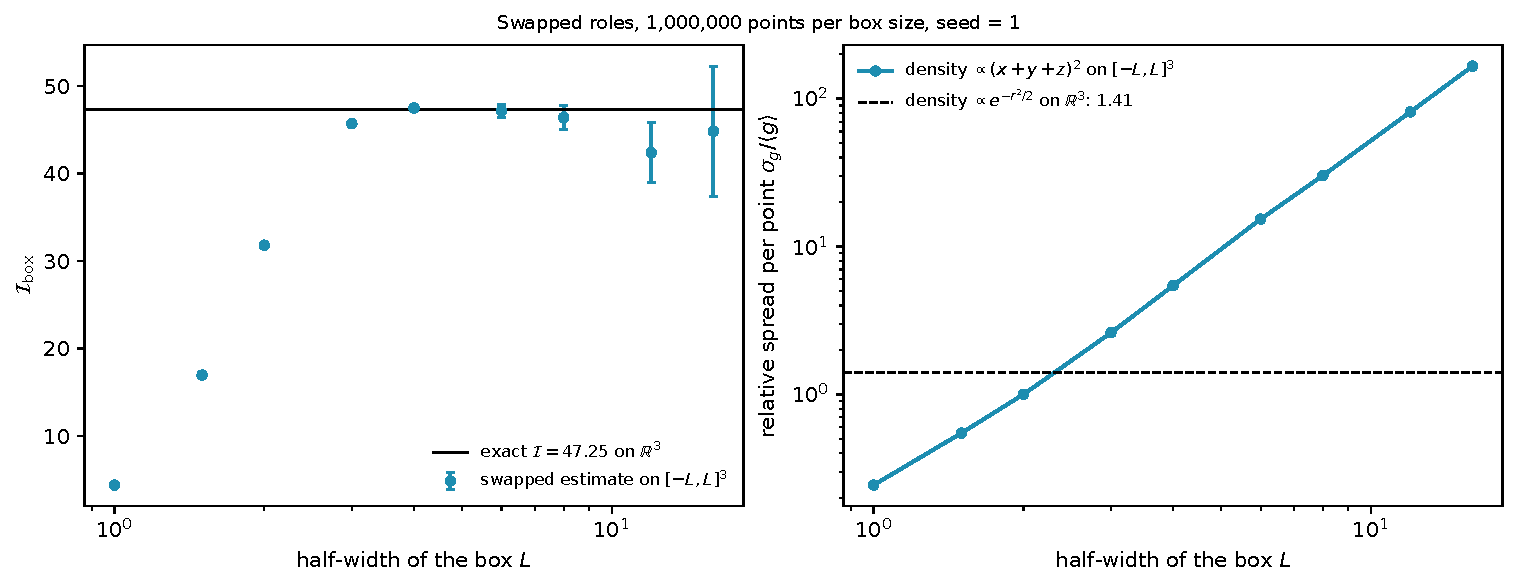
\includegraphics[width=\linewidth]{4.03-mc-integration-1/figures/mc_swapped}
  \caption{Swapped roles, density $\propto(x+y+z)^2$ on $[-L,L]^3$, $10^6$ points per box size
    (seed 1). Left: estimate of the box integral against $L$, with the exact $\mathcal I$ on
    $\mathbb R^3$. Right: relative spread per point $\sigma_g/\avg g$, compared with the Gaussian
    density (dashed).}
  \label{fig:4.3-swapped}
\end{figure}
